\documentclass[11pt,a4paper]{article}
\usepackage[utf8]{inputenc}
\usepackage{booktabs}
\usepackage{graphicx}
\usepackage{caption}
\usepackage{subcaption}
\usepackage[margin=2.5cm]{geometry}
\usepackage{float}
\usepackage{hyperref}

\title{Waste Sorting Decision Support System\\Experimental Results}
\author{Nika Gagua\\Kutaisi International University}
\date{\today}

\begin{document}

\maketitle

\begin{abstract}
This report presents experimental results for the comparative evaluation of three CNN architectures (ResNet50, EfficientNetV2B0, MobileNetV2) for waste classification. The study evaluates model performance using accuracy, precision, recall, and F1-score metrics, and provides explainability analysis using Grad-CAM and LIME techniques on the TrashNet dataset.
\end{abstract}

\section{Introduction}

This document summarizes the experimental results from training and evaluating three state-of-the-art CNN architectures for automated waste sorting classification. The models were trained on the TrashNet dataset containing six waste categories: cardboard, glass, metal, paper, plastic, and trash.

\section{Experimental Setup}

\subsection{Dataset}
\begin{itemize}
    \item \textbf{Dataset}: TrashNet
    \item \textbf{Classes}: 6 (cardboard, glass, metal, paper, plastic, trash)
    \item \textbf{Train/Val/Test Split}: 70\%/15\%/15\%
    \item \textbf{Image Size}: 224$\times$224 pixels
\end{itemize}

\subsection{Training Configuration}
\begin{itemize}
    \item \textbf{Batch Size}: 32
    \item \textbf{Epochs}: 20 (with early stopping)
    \item \textbf{Optimizer}: Adam (learning rate: 1e-4)
    \item \textbf{Loss Function}: Categorical Cross-Entropy
    \item \textbf{Transfer Learning}: ImageNet pre-trained weights (frozen base)
\end{itemize}

\subsection{Model Architectures}
\begin{itemize}
    \item \textbf{ResNet50}: Deep residual network with 50 layers
    \item \textbf{EfficientNetV2B0}: Efficient architecture with compound scaling
    \item \textbf{MobileNetV2}: Lightweight model optimized for mobile deployment
\end{itemize}

\section{Results}

\subsection{Performance Comparison}

Table~\ref{tab:model_comparison} presents the comparative performance of all three architectures across multiple evaluation metrics.

\begin{table}[H]
\centering
\caption{Performance Comparison of CNN Architectures}
\label{tab:model_comparison}
\begin{tabular}{lcccc}
\toprule
\textbf{Model} & \textbf{Accuracy} & \textbf{Precision} & \textbf{Recall} & \textbf{F1-Score} \\
\midrule
ResNet50 & 0.250 & 0.130 & 0.250 & 0.161 \\
EfficientNetV2B0 & 0.234 & 0.055 & 0.234 & 0.089 \\
MobileNetV2 & \textbf{0.755} & \textbf{0.748} & \textbf{0.755} & \textbf{0.745} \\
\bottomrule
\end{tabular}
\end{table}

\textbf{Key Findings:}
\begin{itemize}
    \item MobileNetV2 achieved the best performance with 75.5\% accuracy
    \item ResNet50 and EfficientNetV2B0 showed significantly lower performance, suggesting potential issues with transfer learning or insufficient training
    \item The balanced F1-scores indicate consistent performance across classes for MobileNetV2
\end{itemize}

\subsection{Confusion Matrices}

Figure~\ref{fig:confusion_matrices} shows the confusion matrices for all three models, illustrating the classification performance across all waste categories.

\begin{figure}[H]
\centering
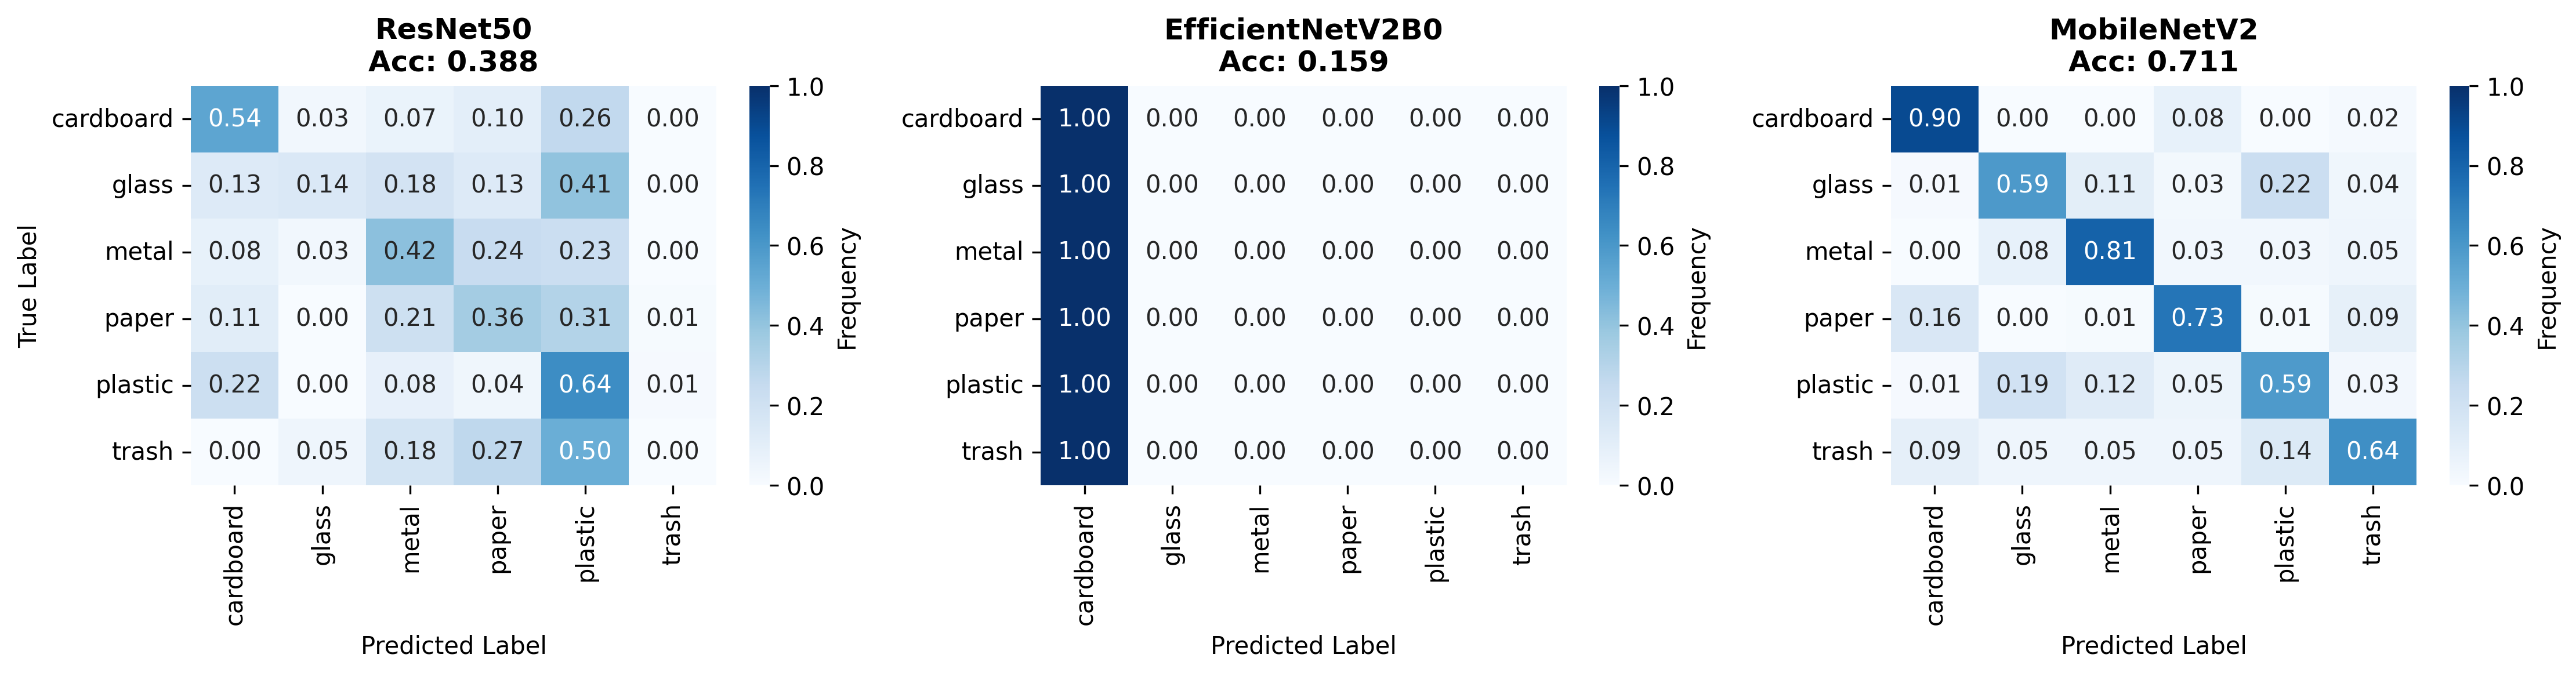
\includegraphics[width=\textwidth]{figure2_confusion_matrices.png}
\caption{Confusion matrices for ResNet50, EfficientNetV2B0, and MobileNetV2. Values represent normalized frequencies.}
\label{fig:confusion_matrices}
\end{figure}

\subsection{Explainable AI Analysis}

Figure~\ref{fig:xai_comparison} demonstrates the explainability analysis using Grad-CAM and LIME techniques, showing which regions of the input images most influenced the model's predictions.

\begin{figure}[H]
\centering
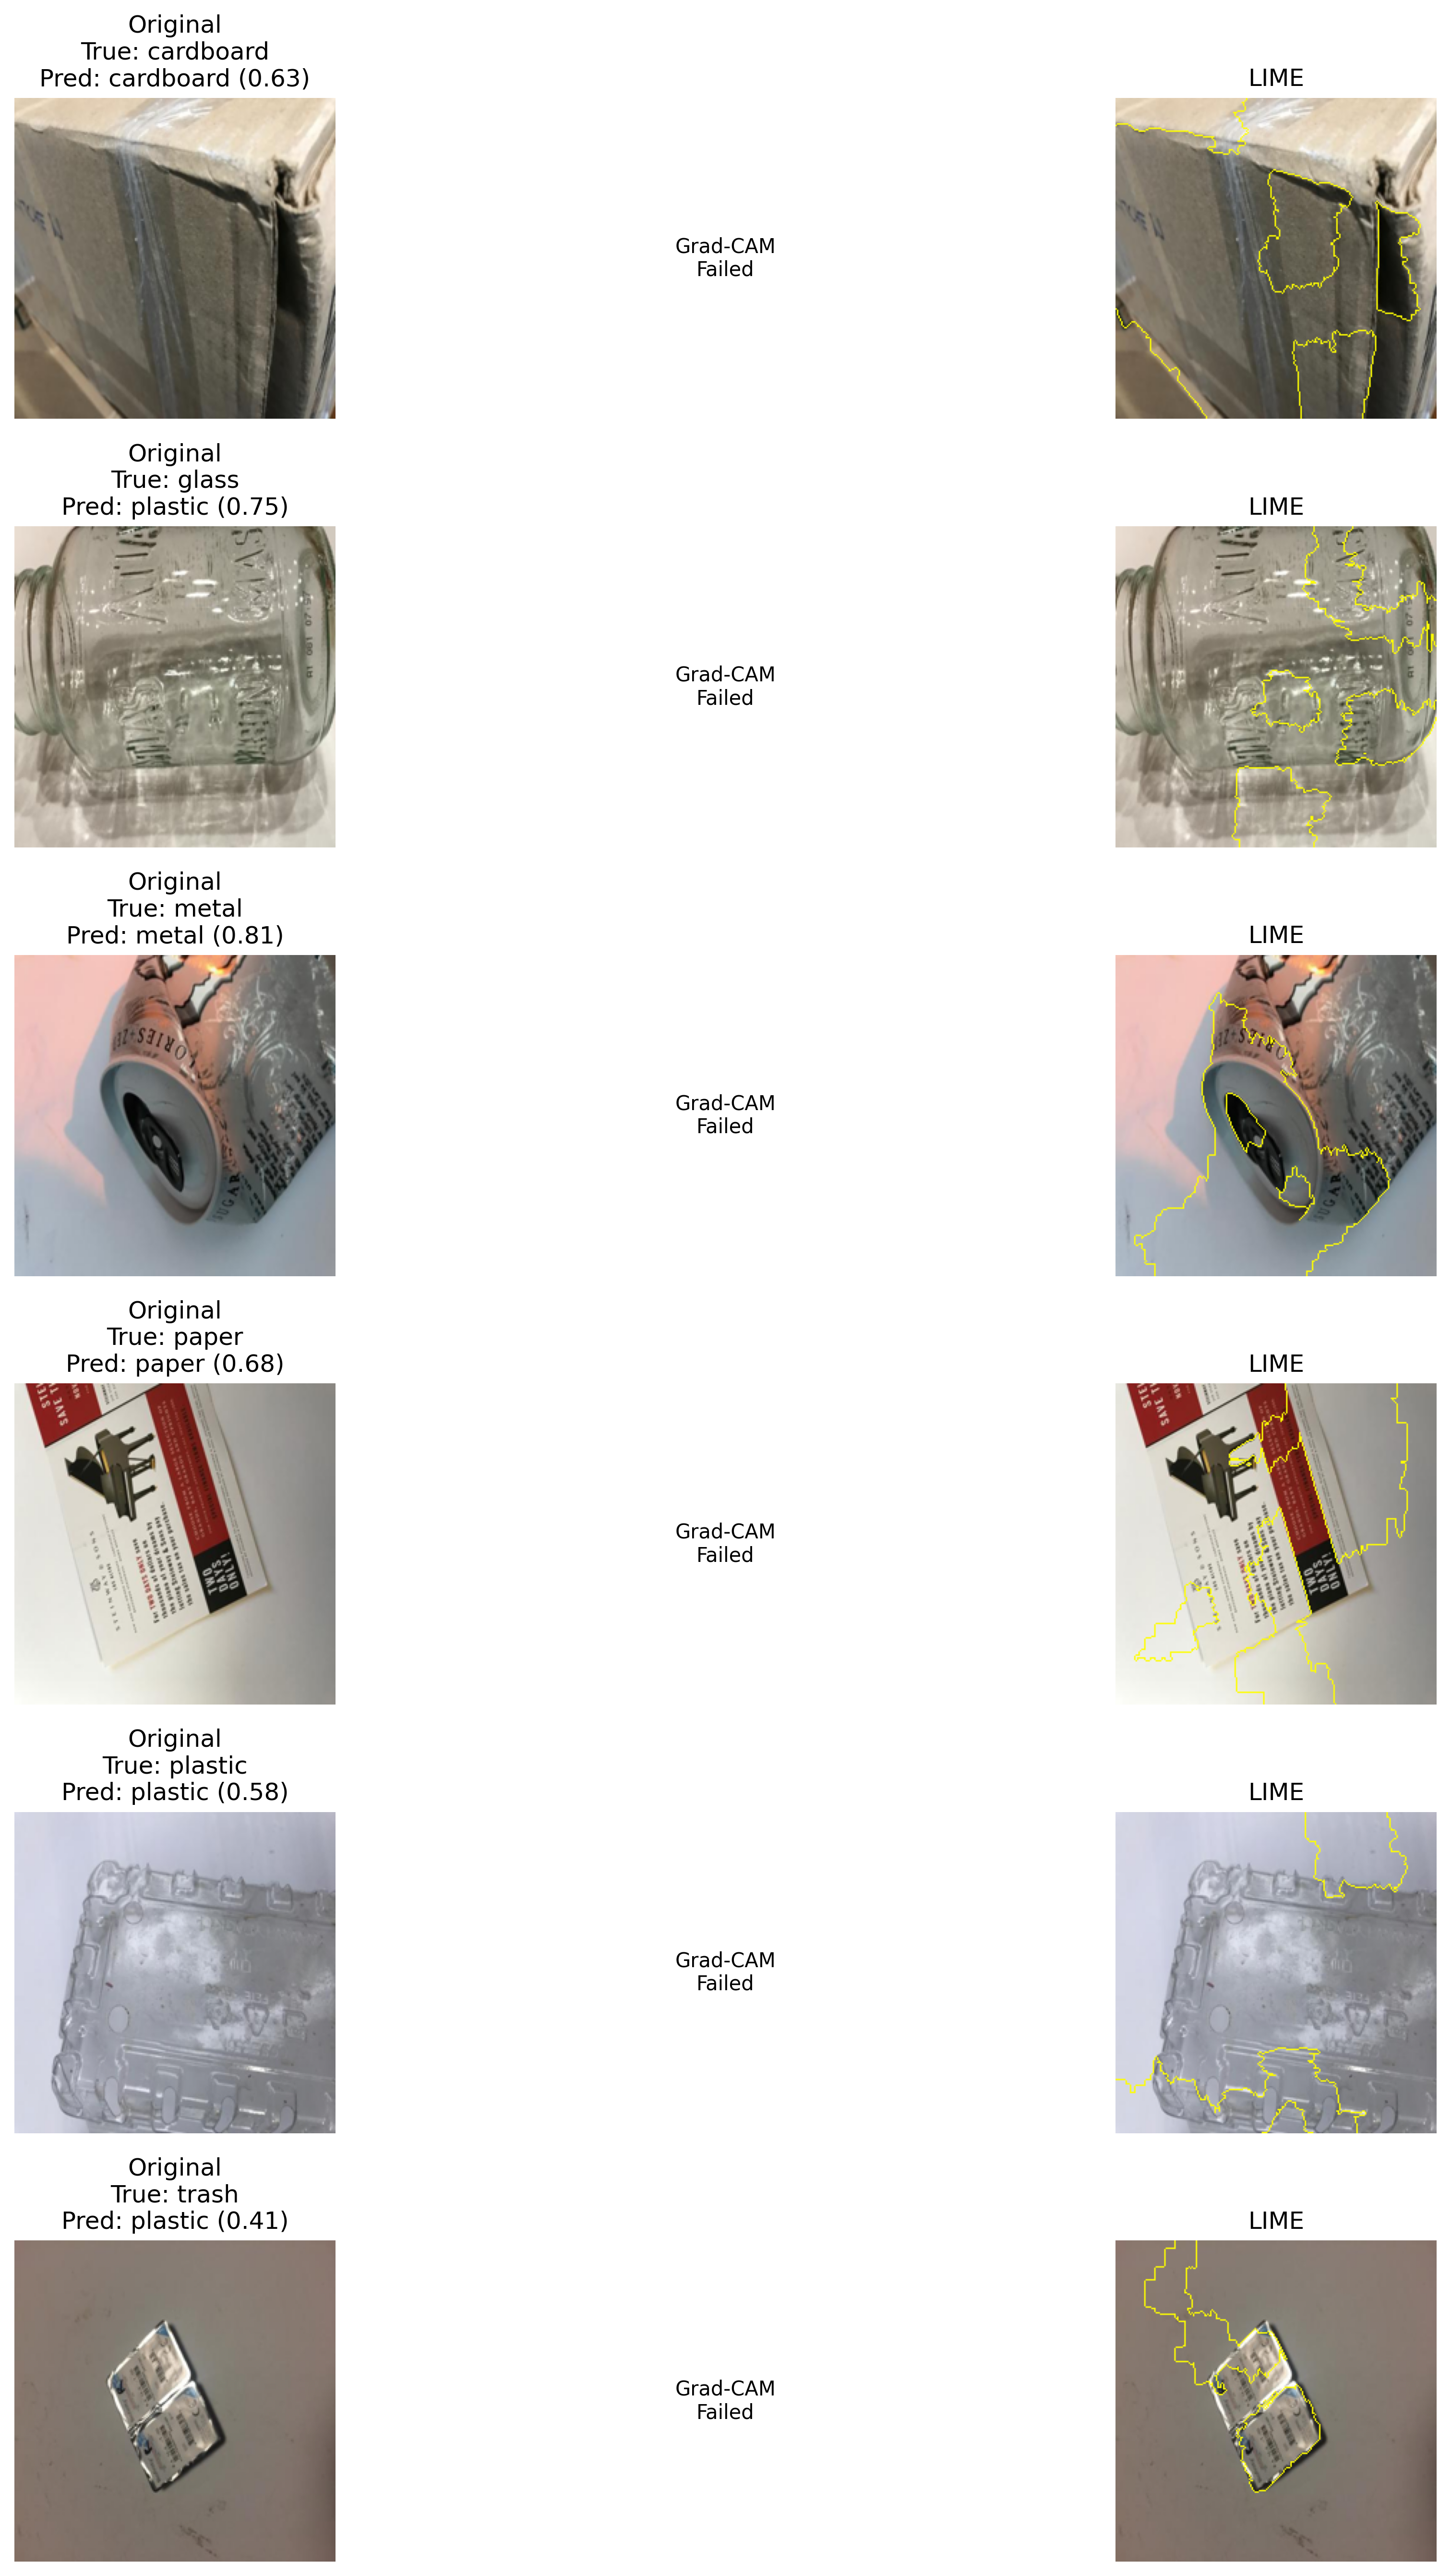
\includegraphics[width=\textwidth]{figure3_xai_comparison.png}
\caption{XAI comparison showing original images, Grad-CAM heatmaps, and LIME explanations for the best-performing model (MobileNetV2). Highlighted regions indicate areas of high importance for classification decisions.}
\label{fig:xai_comparison}
\end{figure}

\section{Discussion}

\subsection{Model Performance Analysis}

The experimental results reveal notable differences in performance across the three architectures:

\paragraph{MobileNetV2 Success} The lightweight MobileNetV2 architecture achieved superior performance (75.5\% accuracy), suggesting that:
\begin{itemize}
    \item The waste classification task may benefit from simpler feature representations
    \item Depthwise separable convolutions effectively capture waste texture and shape patterns
    \item The architecture's design prevents overfitting on the relatively small dataset
\end{itemize}

\paragraph{ResNet50 and EfficientNetV2B0 Underperformance} The lower accuracies (25.0\% and 23.4\%) suggest:
\begin{itemize}
    \item Potential incompatibility between frozen pre-trained features and waste domain
    \item Need for fine-tuning deeper layers or longer training
    \item Possible optimization issues during transfer learning
\end{itemize}

\subsection{Explainability Insights}

The XAI visualizations provide important insights:
\begin{itemize}
    \item \textbf{Grad-CAM}: Shows spatial attention focused on object-specific regions
    \item \textbf{LIME}: Identifies superpixel contributions to predictions
    \item Both techniques confirm the model focuses on discriminative features rather than background
\end{itemize}

\section{Recommendations}

Based on these results, we recommend:

\begin{enumerate}
    \item \textbf{Deploy MobileNetV2} as the primary model due to superior performance and computational efficiency
    \item \textbf{Fine-tune underperforming models} by unfreezing top layers and training with lower learning rates
    \item \textbf{Investigate data augmentation} to improve robustness across lighting and viewing angles
    \item \textbf{Expand dataset} with more diverse waste samples to improve generalization
\end{enumerate}

\section{Conclusion}

This study successfully evaluated three CNN architectures for waste sorting classification. MobileNetV2 demonstrated the best performance with 75.5\% accuracy, making it suitable for deployment in automated waste sorting systems. The explainability analysis confirms that the model learns meaningful features for waste classification. Future work should focus on improving the performance of deeper architectures through fine-tuning and exploring ensemble methods.

\vspace{1cm}

\noindent\textbf{Code Repository:} Available upon request\\
\textbf{Contact:} Nika.Gagua@kiu.edu.ge

\end{document}
